%%%%%%%%%%%%%%%%%%%%%%%%%%%%%%%%%%%%%%%%%%%%%%%%%%%%%%%%%%%%%%%%%%%%
%%%           Vorlage für eine Ausarbeitung an der DHBW          %%%
%%%                                                              %%%
%%%      Bereiche die bearbeitet werden müssen werden durch      %%%
%%%      einen solchen Kommentarblock eingeleitet und enden      %%%
%%%      mit der nächsten Trennlinie.                            %%%
%%%                                                              %%%
%%%      In dieser Datei müssen folgende Bereiche bearbeitet     %%%
%%%      werden:                                                 %%%
%%%      - Angaben zur Arbeit                                    %%%
%%%      - EIGENE KAPITEL EINFÜGEN                               %%%
%%%                                                              %%%
%%%      Benötigte Seiten und Verzeichnisse können unter         %%%
%%%      "Einführung und Verzeichnisse" ein- bzw. auskommentiert %%%
%%%      werden.                                                 %%%
%%%                                                              %%%
%%%%%%%%%%%%%%%%%%%%%%%%%%%%%%%%%%%%%%%%%%%%%%%%%%%%%%%%%%%%%%%%%%%%

\documentclass[a4paper,12pt]{article}
\usepackage[left=2.5cm,right=2.5cm,top=2.5cm,bottom=2.5cm,includehead]{geometry}      % Einstellungen der Seitenränder
\usepackage[english, ngerman]{babel}                                                  % deutsche Silbentrennung
\usepackage[utf8]{inputenc}                                                           % Umlaute
\usepackage[official]{eurosym}                                                        % Euro Symbol
\usepackage[T1]{fontenc}													                                    % Umlaute auch richtig ausgeben
\usepackage{newtxtext,newtxmath}                                                      % Font = Times New Roman
\usepackage{hyperref}
\usepackage{xr-hyper}
\usepackage[nottoc]{tocbibind}
\usepackage{fancyhdr}
\usepackage{setspace}
\usepackage[backend=bibtex, citestyle=authoryear, bibstyle=authoryear]{biblatex}      % Bibliothek für Zitate
\usepackage{csquotes}                                                                 % Zusatzpacket für Zitate
\usepackage{amsmath}                                                                  % Zurücksetzen der Tabellen- und Abbildungsnummerierung je Sektion
\usepackage[labelfont=bf,aboveskip=1mm]{caption}                                      % Bild- und Tabellenunterschrift (fett)
\usepackage[bottom,multiple,hang,marginal]{footmisc}                                  % Fußnoten [Ausrichtung unten, Trennung durch Seperator bei mehreren Fußnoten]
\usepackage{graphicx}  
\graphicspath{{./images/}}                                                            % Grafiken
\usepackage[dvipsnames]{xcolor}                                                       % Farbige Buchstaben
\usepackage{wrapfig}                                                                  % Bilder in Text integrieren
\usepackage{enumitem}                                                                 % Befehl setlist (Zeilenabstand für itemize Umgebung auf 1 setzen)
\usepackage{listings}                                                                 % Quelltexte
\definecolor{commentgreen}{RGB}{87,166,74}                                            % Kommentar-Farbe für Quellcode
\lstset{numbers=left, numberstyle=\tiny, numbersep=8pt, frame=single, framexleftmargin=15pt, breaklines=true, commentstyle=\color{commentgreen}}
\usepackage{tabularx}                                                                 % Tabellen
\usepackage{multirow}                                                                 % Mehrzeilige Tabelleneinträge
\usepackage[addtotoc]{abstract}                                                       % Abstract
\usepackage[nohyperlinks, printonlyused, withpage]{acronym}                           % Abkürzungen
\usepackage{dirtree}                                                                  % Ordnerstruktur (z.B. für Anhang)
\usepackage{pdfpages}                                                                 % PDFs einbinden


%%%%%%%%%%%%%%%%%%%%%%%%%%%%%%%%%%%%%%%%%%%%%%%%%%%%%%%%%%%%%%%%%%%%
%%%                      Angaben zur Arbeit                      %%%
%%%%%%%%%%%%%%%%%%%%%%%%%%%%%%%%%%%%%%%%%%%%%%%%%%%%%%%%%%%%%%%%%%%%
\def\vFirmenlogoPfad{}                  %% relativer Pfad Bsp.: images/Firmenlogo.png
\def\vDHBWLogoPfad{images/DHBW_logo.jpg}                          %% relativer Pfad Bsp.: images/DHBW_logo.jpg
\def\vUnterschrift{}                    %% Pfad zu Bild mit Unterschrift (für digitale Abgabe) Bsp.: images/Unterschrift.png

\def\vTitel{}                           %%
\def\vUntertitel{}                      %%
\def\vArbeitstyp{}                      %% Projektarbeit/Seminararbeit/Bachelorarbeit
\def\vArbeitsbezeichnung{}              %% T1000/T2000/T3000

\def\vAutor{}                           %% Vorname Nachname
\def\vMatrikelnummer{}                  %% 7-stellige Zahl
\def\vKursKuerzel{}                     %% Bsp.: TIT20
\def\vPhasenbezeichnung{}               %% Praxisphase/Theoriephase
\def\vStudienJahr{}                     %% erste/zweite/dritte
\def\vDHBWStandort{}                    %% Bsp.: Ravensburg
\def\vDHBWCampus{}                      %% Bsp.: Friedrichshafen
\def\vFakultaet{}                       %% Technik/Wirtschaft
\def\vStudiengang{}                     %% Informationstechnik/...

\def\vBetrieb{}                         %%
\def\vBearbeitungsort{}                 %%
\def\vAbteilung{}                       %%
\def\vBetreuer{}                        %% Vorname Nachname

\def\vAbgabedatum{\today}               %% DD. MONTH YYYY
\def\vBearbeitungszeitraum{}            %% DD.MM.YYYY - DD.MM.YYYY


%%%%%%%%%%%%%%%%%%%%%%%%% Eigene Kommandos %%%%%%%%%%%%%%%%%%%%%%%%%
% Definition von \gqq{} und \gq{}: Text in Anführungszeichen
\newcommand{\gqq}[1]{\glqq #1\grqq}
\newcommand{\gq}[1]{\glq #1\grq}
% Spezielle Hervorhebung von Schlüsselwörtern
\newcommand{\textOrdner}[1]{\texttt{#1}}
\newcommand{\textVariable}[1]{\texttt{#1}}
\newcommand{\textKlasse}[1]{\texttt{#1}}
\newcommand{\textFunktion}[1]{\texttt{#1}}


%%%%%%%%%%%%%%%%%%%% Zitatbibliothek einbinden %%%%%%%%%%%%%%%%%%%%%
\addbibresource{literatur/literatur.bib}
\addbibresource{literatur/Noel.bib}


%%%%%%%%%%%%%%%%%%%%%%%% PDF-Einstellungen %%%%%%%%%%%%%%%%%%%%%%%%%
\hypersetup{
  bookmarksopen=false,
	bookmarksnumbered=true,
	bookmarksopenlevel=0,
  pdftitle=\vTitel,
  pdfsubject=\vTitel,
  pdfauthor=\vAutor,
  pdfborder={0 0 0},
	pdfstartview=Fit,
  pdfpagelayout=SinglePage
}


%%%%%%%%%%%%%%%%%%%%%%%% Kopf- und Fußzeile %%%%%%%%%%%%%%%%%%%%%%%%
\pagestyle{fancy}
\setlength{\headheight}{15pt}
\fancyhf{}
\fancyhead[R]{\thepage}


%%%%%%%%%%%%%%%%%%%%%%%%%%%%%% Layout %%%%%%%%%%%%%%%%%%%%%%%%%%%%%%
\onehalfspacing
\setlist{noitemsep}

\addto\captionsngerman{
  \renewcommand{\figurename}{Abb.}
  \renewcommand{\tablename}{Tab.}
}
\numberwithin{table}{section}                               % Tabellennummerierung je Sektion zurücksetzen
\numberwithin{figure}{section}                              % Abbildungsnummerierung je Sektion zurücksetzen
\renewcommand{\thetable}{\arabic{section}.\arabic{table}}   % Tabellennummerierung mit Section
\renewcommand{\thefigure}{\arabic{section}.\arabic{figure}} % Abbildungsnummerierung mit Section
\renewcommand{\thefootnote}{\arabic{footnote}}              % Sektionsbezeichnung von Fußnoten entfernen

\renewcommand{\multfootsep}{, }                             % Mehrere Fußnoten durch ", " trennen


%%%%%%%%%%%%%%%%%%%%%%%%%%%%% Dokument %%%%%%%%%%%%%%%%%%%%%%%%%%%%%

\begin{document}


  %%%%%%%%%%%%%%%%%%% Einführung und Verzeichnisse %%%%%%%%%%%%%%%%%%%
  \pagenumbering{Roman}

  \begin{titlepage}
  \begin{minipage}{6in}
    \vspace*{-2cm}
    \centering
    \hspace{-2cm}
	\ifx\vFirmenlogoPfad\empty
	\else
    \raisebox{-0.5\height}{\includegraphics[height=4cm]{\vFirmenlogoPfad}}
  \fi
	\hfill
	\ifx\vDHBWLogoPfad\empty
	\else
   	\raisebox{-0.5\height}{\includegraphics[height=4cm]{\vDHBWLogoPfad}}
	\fi
  \end{minipage}
  \begin{center}
    \vspace*{0.5cm}
    \Huge\textbf{\vTitel}\\
		\ifx\vUntertitel\empty
		\else
			\Large\rm\vUntertitel\\
		\fi
		\vspace*{2cm}
		\Large\textbf{\vArbeitstyp}
		\ifx\vArbeitsbezeichnung\empty
		\else
			\textbf{\vArbeitsbezeichnung}
		\fi
		\\
		\normalsize
		über die \vPhasenbezeichnung\ des \vStudienJahr{n}\ Studienjahrs \\
		\vspace*{1cm}
		an der Fakultät für \vFakultaet\\
		im Studiengang \vStudiengang\\
		\vspace*{0.5cm}
		an der DHBW \vDHBWStandort\\
		\ifx\vDHBWCampus\empty
		\else
		Campus \vDHBWCampus\\
		\fi
		\vspace*{0.5cm}
		von\\
		\ifx\vAutor\empty
		\else
			\vAutor\\
		\fi
		\vspace*{1cm}
		\vAbgabedatum
		\vfill
  \end{center}
  \begin{tabular}{ll}
    Bearbeitungszeitraum:&\vBearbeitungszeitraum\\
    Matrikelnummer, Kurs:&\vMatrikelnummer, \vKursKuerzel\\
	  Dualer Partner:&\vBetrieb\\
	  Betreuer des Dualen Partners:&\vBetreuer\\
  \end{tabular}
\end{titlepage}
\newpage
\setcounter{page}{2}
  % \thispagestyle{empty}
\section*{\Huge{Sperrvermerk}}

\addcontentsline{toc}{section}{Sperrvermerk}
gemäß Ziffer 1.1.13 der Anlage 1 zu §§ 3, 4 und 5  der Studien- und Prüfungsordnung für die Bachelorstudiengänge im Studienbereich Technik der Dualen Hochschule Baden-Würt­tem­berg vom 29.09.2017.\\

\noindent \gqq{Der Inhalt dieser Arbeit darf weder als Ganzes noch in Auszügen Personen außerhalb des Prüfungsprozesses und des Evaluationsverfahrens zugänglich gemacht werden, sofern keine anders lautende Genehmigung vom Dualen Partner vorliegt.}

\vfill
\leavevmode
\newline
\parbox{6cm}{\strut\centering \vBearbeitungsort, \vAbgabedatum\hrule\strut\centering\footnotesize Ort, Datum} 
\hfill
\ifx\vUnterschrift\empty
\parbox{6cm}{\strut\hspace{1pt} \vAbteilung\hrule\strut\centering\footnotesize Abteilung, Unterschrift}
\else
\parbox{6cm}{\strut\hspace{1pt} \vAbteilung, \parbox[b]{3cm}{\vspace{-10cm}\includegraphics[width=3cm]{\vUnterschrift}}\hrule\strut\centering\footnotesize Abteilung, Unterschrift}
\fi
\vspace{1cm}

\newpage
  \thispagestyle{empty}
\section*{\Huge{Selbstständigkeitserklärung}}

\addcontentsline{toc}{section}{Selbstständigkeitserklärung}
gemäß Ziffer 1.1.13 der Anlage 1 zu §§ 3, 4 und 5  der Studien- und Prüfungsordnung für die Bachelorstudiengänge im Studienbereich Technik der Dualen Hochschule Baden-Würt­tem­berg vom 29.09.2017.

\noindent Ich versichere hiermit, dass ich meine Bachelorarbeit (bzw. Projektarbeit oder Studienarbeit bzw. Hausarbeit) mit dem Thema: 
\begin{center}
	\Large\textbf{\vTitel}
\end{center}
selbstständig verfasst und keine anderen als die angegebenen Quellen und Hilfsmittel benutzt habe. Ich versichere zudem, dass die eingereichte elektronische Fassung mit der gedruckten Fassung übereinstimmt.

\vfill
\leavevmode

\parbox{6cm}{\strut\centering \vBearbeitungsort, \vAbgabedatum\hrule\strut\centering\footnotesize Ort, Datum} 
\hfill
\ifx\vUnterschrift\empty
\parbox{6cm}{\strut\hspace{1pt} \vAbteilung, \hrule\strut\centering\footnotesize Tobias Götz}
\else
\parbox{6cm}{\strut\hspace{1pt} \vAbteilung, \parbox[b]{3cm}{\vspace{-10cm}\includegraphics[width=3cm]{\vUnterschrift}}\hrule\strut\centering\footnotesize Tobias Götz}
\fi
\vspace{1cm}

\parbox{6cm}{\strut\centering \vBearbeitungsort, \vAbgabedatum\hrule\strut\centering\footnotesize Ort, Datum}
\hfill
\ifx\vUnterschriftKempter\empty
\parbox{6cm}{\strut\hspace{1pt} \vAbteilung, \hrule\strut\centering\footnotesize Noel Kempter}
\else
\parbox{6cm}{\strut\hspace{1pt} \vAbteilung, \parbox[b]{3cm}{\vspace{-10cm}\includegraphics[width=3cm]{\vUnterschriftKempter}}\hrule\strut\centering\footnotesize Noel Kempter}
\fi
\vspace{1cm}

\parbox{6cm}{\strut\centering \vBearbeitungsort, \vAbgabedatum\hrule\strut\centering\footnotesize Ort, Datum}
\hfill
\ifx\vUnterschriftKuest\empty
\parbox{6cm}{\strut\hspace{1pt} \vAbteilung, \hrule\strut\centering\footnotesize Philipp Küst}
\else
\parbox{6cm}{\strut\hspace{1pt} \vAbteilung, \parbox[b]{3cm}{\vspace{-10cm}\includegraphics[width=3cm]{\vUnterschriftKuest}}\hrule\strut\centering\footnotesize Philipp Küst}
\fi
\vspace{1cm}

\newpage
  \phantomsection
\newenvironment{keywords}{
	\begin{flushleft}
	\small	
	\textbf{
		\iflanguage{ngerman}{Schlüsselwörter}{\iflanguage{english}{Keywords}{}}
	}
}{\end{flushleft}}

% Deutsche Zusammenfassung
\begin{abstract}
	
\end{abstract}

% Schlüsselwörter Deutsch
\begin{keywords}
	
\end{keywords}


\selectlanguage{english}
% Englisches Abstract
\begin{abstract}

\end{abstract}

% Schlüsselwörter Englisch
\begin{keywords}

\end{keywords}


\selectlanguage{ngerman}
\newpage
  \tableofcontents
\newpage
  \section*{Abkürzungsverzeichnis}
\addcontentsline{toc}{section}{Abkürzungsverzeichnis}
\begin{acronym}
  \acro{DHBW}[DHBW]{Duale Hochschule Ba\-den-\-Würt\-tem\-berg}
  \acroplural{DHBW}[DHBW]{Dualen Hochschule Ba\-den-\-Würt\-tem\-berg}
\end{acronym}
\newpage
  \listoffigures
\newpage
  \listoftables
\newpage
  \lstlistoflistings
\addcontentsline{toc}{section}{Listings}
\newpage
  % \section*{Vorwort}
\addcontentsline{toc}{section}{Vorwort}
\newpage


  %%%%%%%%%%%%%%%%%%%%%%%%%%%%% Kapitel %%%%%%%%%%%%%%%%%%%%%%%%%%%%%%
  \pagestyle{fancy}
  \fancyhead[L]{\nouppercase{\rightmark}}    % Abschnittsname im Header
  \pagenumbering{arabic}

  %%%%%%%%%%%%%%%%%%%%%%%%%%%%%%%%%%%%%%%%%%%%%%%%%%%%%%%%%%%%%%%%%%%%
  %%%%                   EIGENE KAPITEL EINFÜGEN                  %%%%
  %%%%%%%%%%%%%%%%%%%%%%%%%%%%%%%%%%%%%%%%%%%%%%%%%%%%%%%%%%%%%%%%%%%%
  \section{Einleitung}
\subsection{Aufgabenstellung}
Im Rahmen dieser Hausarbeit soll eine Anforderungsanalyse für ein Softwareprojekt durchgeführt werden.
Dabei soll ein Video-on-Demand System entwickelt werden, welches es ermöglicht, Videos über das Internet anzusehen.
Dies soll in Anlehnung an die Webseite \url{https://www.primevideo.com} erfolgen.
Einschränkend ist dabei zu erwähnen, dass ausschließlich aktuelle Kinofilme angeboten werden sollen.
Ältere Filme oder Serien sollen somit nicht vom System angeboten werden.

\subsection{Aufbau der Arbeit}
Dieses Dokument ist in zwei Teile aufgeteilt.
Im ersten Teil wird auf die wissenschaftliche Herangehensweise an die Anforderungsanalyse eingegangen.
Hierzu werden die einzelnen Aspekte einer Anforderungsanalyse beschrieben und die einzelnen Methoden, welche in der Anforderungsanalyse verwendet werden, erklärt.
Dies wird mit wissenschaftlichen Quellen untermauert, um die allgemeine Qualität dieser Anforderungsanalyse zu gewährleisten.

Der zweite Teil beschreibt die praktische Umsetzung der Anforderungsanalyse des Video-on-Demand Systems.
Auf Basis der in Teil 1 beschriebenen Methoden wird Schritt für Schritt erklärt, wie die Ergebnisse der Anforderungsanalyse entstanden sind.
Der Fokus hierbei liegt auf den erarbeiteten Anforderungen, auf welche im Text zwar eingegangen wird, jedoch nicht im Detail.
Der gesamte Anforderungskatalog befindet sich im Anhang, um eine bessere Übersichtlichkeit zu gewährleisten.
Auf diese Weise kann der Leser die Anforderungen nachlesen, ohne den Text zu stören.

  \externaldocument{anhang}
\subsection{Ereignisgesteuerte Prozesskette (EPK)}\label{subsec:epk)}
Ereignisgesteuerte Prozessketten sind seit ihrer Entwicklung im Jahr 1992 eine beliebte und weitverbreitete Methode zur 
Geschäftsprozessmodellierung (vgl. \autocite{epc-diagram}).
Grund hierfür ist die geringe Zeit, die für die Erstellung dieser Diagramme benötigt wird.
Des Weiteren sind EPK-Modelle übersichtlich und leicht verständlich.
Damit eignen sie sich ideal um im Rahmen des Requirements Engineering die Kernprozesse einer Anwendung zu modellieren.
Anhand dieser Modelle können anschließend Anforderungen an die Anwendung abgeleitet werden.
Aus diesen Gründen wurden im Rahmen dieser Arbeit einige EPK-Modelle erstellt (siehe \nameref{subsec:epk-modelle}), um den Prozess der Anforderungserstellung zu unterstützen.
Da es keine eindeutig zentralisierte schreibweise für EPK-Modelle gibt, wurde ebenfalls eine Legende der verwendeten Konventionen beigefügt (siehe \nameref{fig:epk_legende}).

  \subsection{Das Kano-Modell}\label{subsec:kano-modell}
Für eine erfolgreiche Anforderungsanalyse ist es notwendig die Anforderungen an die Anwendung nicht nur zu erfassen,
sondern diese auch zu kategorisieren.
Dies ermöglicht es bei der anschließenden Entwicklung des Systems Anforderungen nach ihrer Priorität abzuarbeiten.
Im Rahmen dieser Arbeit wurde das Kano-Modell verwendet, um die erhobenen Anforderungen zu kategorisieren.
Wie Abbildung~\nameref{fig:kano_model} zeigt handelt es sich um ein Modell, welches die Erfüllung von Anforderungen mit
der Kundenzufriedenheit in Beziehung setzt.

\begin{figure}[ht]
    \centering
    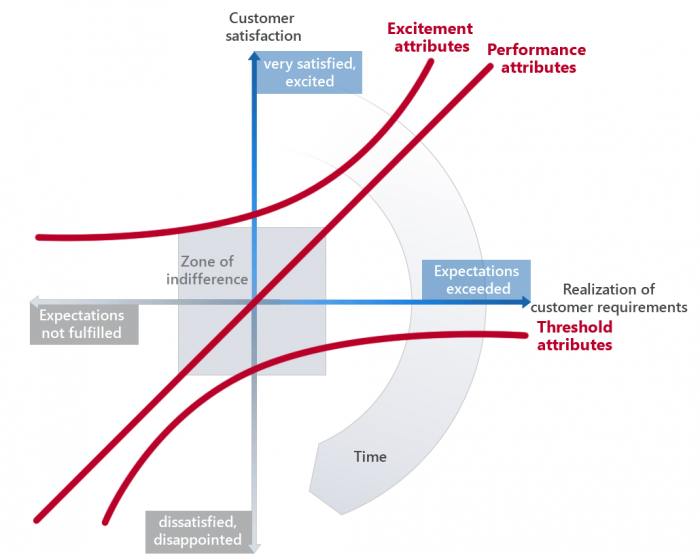
\includegraphics[width=0.8\textwidth]{images/Kano-Model}
    \caption{Kano-Modell~\autocite{kano-model}}
    \label{fig:kano_model}
\end{figure}

Die Anforderungen werden dabei in fünf Kategorien eingeteilt:

\begin{itemize}
    \item \textbf{Basisfaktoren:} Werden als selbstverständlich angesehen und führen bei fehlender Umsetzung für Unzufriedenheit
    \item \textbf{Leistungsfaktoren:} Werden vom Stakeholder explizit gefordert und führen zu Zufriedenheit bei Umsetzung
    und Unzufriedenheit bei Nichtumsetzung
    \item \textbf{Begeisterungsfaktoren:} Werden nicht explizit vom Stakeholder gefordert und führen auch nicht zu Unzufriedenheit
    bei Nichtumsetzung, steigern jedoch die Zufriedenheit bei Umsetzung
    \item \textbf{Gleichgültige Qualitäten:} Haben weder einen positiven noch einen negativen Einfluss auf die Kundenzufriedenheit,
    egal ob sie umgesetzt werden oder nicht
    \item \textbf{Umgekehrte Qualitäten:} Führen zu Unzufriedenheit bei Umsetzung aber nicht zu Zufriedenheit bei Nichtumsetzung
\end{itemize} (vgl.~\autocite{kano-model})
Wichtig zu beachten ist der Einfluss der Zeit auf die Kategorisierung der Anforderungen, denn mit fortschreitender Zeit werden
aus Begeisterungsfaktoren Leistungsfaktoren und aus Leistungsfaktoren Basisfaktoren.

\subsection{Anforderungsermittlung}\label{subsec:anforderungsermittlung}
Um Anforderungen kategorisieren zu können, müssen diese allerdings zuerst ermittelt werden.
Hierfür gibt es verschiedene Techniken, welche im Allgemeinen in folgende Kategorien eingeteilt werden können:

\begin{itemize}
    \item \textbf{Befragungstechniken:} Werden in direkter Zusammenarbeit mit dem Stakeholder durchgeführt (z.B.: Interviews, Fragebögen)
    \item \textbf{Kreativtechniken:} Entwicklung innovativer Ideen oder einer ersten groben Lösung (z.B.: Brainstorming, Perspektivenwechsel)
    \item \textbf{Dokumenten- und systembasierte Techniken:} Untersuchung bereits existierender Dokumente und Systeme,
    welche für die Anwendung relevant sind (z.B.: Systemarchäologie)
    \item \textbf{Beobachtungstechniken:} Beobachtung der Stakeholder und ihrer Arbeitsabläufe (z.B.: Feldbeobachtung)
    \item \textbf{Unterstützende Techniken:} Werden ergänzend zu anderen Techniken angewandt (z.B.: Prototyping, Workshops)
\end{itemize} (vgl.~\autocite{Maulhardt.b})

In Kombination mit dem Kano-Modell kommen häufig Befragungstechniken und Kreativtechniken zum Einsatz.
Befragungstechniken ermöglichen es in Zusammenarbeit mit dem Stakeholder Anforderungen zu ermitteln und direkt nach dem
Kano-Modell zu kategorisieren,
und sind damit speziell für die Ermittlung der Leistungsfaktoren geeignet.
Kreativtechniken eignen sich hingegen besonders gut für die Ermittlung von Begeisterungsfaktoren, da diese nicht explizit
von den Stakeholdern gefordert werden.


  %%%%%%%%%%%%%%%%%%%%%%% Literaturverzeichnis %%%%%%%%%%%%%%%%%%%%%%%
  \phantomsection
\addcontentsline{toc}{section}{Literatur}
\printbibliography
\newpage


  %%%%%%%%%%%%%%%%%%%%%%%%%%%%%% Anhang %%%%%%%%%%%%%%%%%%%%%%%%%%%%%%
  \renewcommand{\thetable}{\Alph{section}.\arabic{table}}
  \renewcommand{\thefigure}{\Alph{section}.\arabic{figure}}
  \renewcommand{\thelstlisting}{\Alph{section}.\arabic{lstlisting}}
  \pagenumbering{Alph}

  \begin{appendix}
  \section{Anhang}
\end{appendix}
\end{document}